\documentclass[a4paper,14pt]{extarticle}

\usepackage[T2A]{fontenc}
\usepackage[utf8]{inputenc}
\usepackage[english,russian]{babel}
\usepackage{indentfirst}
\usepackage{setspace}
\usepackage{geometry}
\geometry{a4paper,left=30mm,right=15mm,top=20mm,bottom=20mm}
\onehalfspacing
\setlength{\parindent}{1.25cm}

% Выравнивание заголовков по ГОСТ ИТМО
\usepackage{titlesec}
\titleformat{\section}[block]
{\centering\bfseries\Large}{\thesection}{1em}{}
\titleformat{\subsection}[block]
{\centering\bfseries\large}{\thesubsection}{1em}{}
\titleformat{\subsubsection}[block]
{\centering\bfseries\normalsize}{\thesubsubsection}{1em}{}

% Настройка подписей к рисункам по ГОСТ (номер и текст по центру)
\usepackage{caption}
\captionsetup[figure]{
    justification=centering,
    labelsep=endash,
    font=small,
    name=Рисунок,
    singlelinecheck=true
}

% Нумерация страниц по ГОСТ (снизу по центру)
\usepackage{fancyhdr}
\pagestyle{fancy}
\fancyhf{}
\fancyfoot[C]{\hspace{-15mm}\thepage}
\renewcommand{\headrulewidth}{0pt}

% Формат списков по ГОСТ
\usepackage{enumitem}
\setlist{nosep, leftmargin=1.25cm}
\setlist[itemize]{label=\raisebox{0.3ex}{\tiny$\bullet$}, labelsep=0.5em}

% Ссылки и математика
\usepackage{hyperref}
\hypersetup{
    colorlinks=true,
    linkcolor=black,
    urlcolor=black,
    citecolor=black
}
\usepackage{amsmath}
\usepackage{graphicx}

% Разрешить более свободный перенос длинных строк
\sloppy

% Команды для удобства
\newcommand{\sectionbreak}{\clearpage}
\newcommand{\img}[3]{%
    \begin{figure}[H]
    \centering
    \includegraphics[width=#1\textwidth]{#2}
    \caption{#3}
    \label{fig:#2}
    \end{figure}
}

\begin{document}
    \thispagestyle{empty}
    \begin{center}
    {\Large\textbf{ФЕДЕРАЛЬНОЕ ГОСУДАРСТВЕННОЕ АВТОНОМНОЕ ОБРАЗОВАТЕЛЬНОЕ УЧРЕЖДЕНИЕ ВЫСШЕГО ОБРАЗОВАНИЯ}}
        \\
        {\Large\textbf{«НАЦИОНАЛЬНЫЙ ИССЛЕДОВАТЕЛЬСКИЙ УНИВЕРСИТЕТ ИТМО»}}\\[5mm]
        {\large ФАКУЛЬТЕТ ТЕХНОЛОГИЙ ИСКУССТВЕННОГО ИНТЕЛЛЕКТА}\\[5mm]
        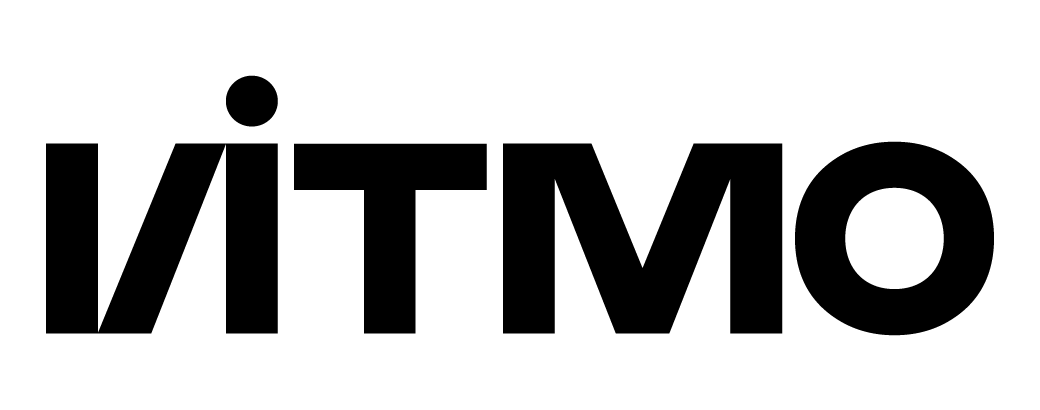
\includegraphics[scale=0.14]{logo.png}\\[10mm]
        \rule{\textwidth}{0.4mm}\\[3mm]
        {\Large Расчётно-графическая работа \textnumero{} 1 }\\[3mm]
        {\Large по дисциплине «Теория вероятностей }\\[3mm]
        {\Large и продвинутая математическая статистика» }\\[3mm]
        \rule{\textwidth}{0.4mm}
    \end{center}
    \vfill
    \begin{flushright}
        \large Выполнили студенты группы J3211: \\
        Воробьев А.П. \\
        ИСУ: 465440 \\
        Шакина А.С. \\
        ИСУ: 465472 \\
        Преподаватель практики: \\
        Кононов И.А.
    \end{flushright}
    \vfill
    \begin{center}
        \large Санкт-Петербург \\
        \large 2025
    \end{center}
    \newpage


% =============================================
% Задача 1
% =============================================
    
    
    \section*{Задача 1}
        
        \subsection*{Постановка задачи}
            
            Требуется аналитически решить задачу. Помимо этого нужно написать программу, которая будет считать данные вероятности приблизительно с помощью метода Монте-Карло. Особо любознательные могут задаться поиском (аналитическим) оптимального количества итераций, которых будет достаточно для получения ответа с достаточно «разумной» точностью. При решении задач могут быть полезны принципы произведения вероятностей и включений-исключений.
        
        \subsection*{Условие варианта 2}
            
            В городе живут \( n + 1 \) людей. Человек, условный «прародитель», пишет два письма случайно выбранным адресатам, которые образуют «первое» поколение. Те делают то же самое, в результате чего образуется «второе поколение». В общем, на каждое полученное письмо горожанин готовит два ответа и отправляет двум случайным жителям. Найти вероятность того, что прародитель не входит ни в одно из поколений с номерами \( 1 \ldots r \).
        
        \subsection*{Аналитическое решение}
            
            \subsubsection*{Обозначения и допущения}
                
                Обозначения:
                \begin{itemize}
                    \item \( n + 1 \) - количество жителей города.
                    \item \( r \) - количество поколений, которые мы рассматриваем.
                    \item \( S_i \) - число входящих писем в поколении \( i \).
                    \item \( A \) - событие, что прародитель не является адресатом письма
                \end{itemize}
                
                Допущение: Отправитель письма не может быть его адресатом.
            
            \subsubsection*{Решение}
                
                Рассмотрим \( i \)-е поколение.
                Каждое входящее письмо порождает два исходящих, которые отправляются двум случайным жителям города (кроме самого отправителя). Так как в первом поколении - \( S_1 = 2 \) письма, то во втором поколении будет \( S_2 = 2 \cdot S_1 = 4 \) и так далее. Таким образом, количество писем в \( i \)-м поколении можно выразить формулой:
                \[
                    S_i = 2 \cdot S_{i-1} = 2^i
                \]

                Заметим, что в первом поколении не может быть прародителя, поэтому количество писем за \( r \) поколений, адресатом для которого может быть прародитель, равно:
                \[
                    M = \sum_{i=2}^{r} S_i = \sum_{i=2}^{r} 2^i = 2^{r+1} - 4
                \]

                Теперь найдем вероятность \( P(A) \), что прародитель не является адресатом одного письма. Так как отправитель не может быть адресатом, то для каждого письма есть \( n \) возможных адресатов, из которых \( n - 1 \) не являются прародителем. Значит:
                \[
                    P(A) = \frac{n - 1}{n}
                \]

                Так как все адресаты выбираются независимо, то вероятность \( P (A_M) \), что прародитель не является адресатом ни одного из \( M \) писем:
                \[
                    P(A_M) = P(A)^M = \left(\frac{n - 1}{n}\right)^{2^{r+1} - 4}
                \]
            
            \subsubsection*{Ответ}
            
                Таким образом, искомая вероятность, что прародитель не входит ни в одно из поколений с номерами \( 1 \ldots r \), равна:
                \[
                    \boxed{P(A_M) = \left(\frac{n - 1}{n}\right)^{2^{r+1} - 4}}
                \]


% =============================================
% Задача 3
% =============================================

    \section*{Задача 3}
        
        \subsection*{Постановка задачи}
            
            Требуется аналитически решить задачу.
        
        \subsection*{Условие варианта 2}
            
            Введём события \( A_i = \{X = i\}, B_i = \{Y = i\}, i \geq 0 \). Известно, что для любых \( i \geq 0, j \geq 0 \) события \( A_i \) и \( B_j \) -- независимы, при этом 
            \[ P(X = i) = e^{-\lambda} \frac{\lambda^i}{i!}, \lambda > 0, i \geq 0, \]
            \[ P(Y = j) = e^{-\mu} \frac{\mu^j}{j!}, \mu > 0, i \geq 0. \]
            Требуется найти \( P(X = i | X + Y = j) \).
        
        \subsection*{Решение}
            
            Для нахождения вероятности \( P(X = i | X + Y = j) \) используем формулу условной вероятности: 
            \[ P(A|B) = \frac{P( A \cap B)}{P(B)}, \]
            причём \(A = \{X = i\}, B = \{X + Y = j\}\). 

            Найдём \(P( A \cap B)\). Пересечение событий означает, что что \(X\) должно быть равно \(i\), и одновременно \(X+Y\) должно быть равно \(j\). Это возможно только если \(Y=j-i\). 

            Таким образом, событие \(\{X = i \cap X + Y = j\}\) эквивалентно событию \(\{X = i \cap Y = j - i\}\). Подставим в формулу:
            \[P(A \cap B ) =  e^{-\lambda} \frac{\lambda^i}{i!} \cdot e^{-\mu} \frac{\mu^{j-i}}{(j-i)!} = e^{-(\lambda + \mu)} \cdot \frac{\lambda^i \mu^{j-i}}{i!(j-i)!}\]

            Найдём \(P(B) = P(X + Y = j) \). Запишем событие \(\{X + Y = j\}\) как \(\{X = k \cap Y = j-k\} \;\; \forall k \in {1, \dots, j}\). Так как события несовместны и независимы: 
            \[ P(X + Y = j) = \sum_{k=0}^{j} P(X = k \cap Y = j-k) = \sum_{k=0}^{j}P(X = k) P(Y = j - k)\]

            По условию: 
            \[P(X = k) = e^{-\lambda} \frac{\lambda^k}{k!}, \; P(Y = j - k) = e^{-\mu} \frac{\mu^{j-k}}{(j-k)!}, \]
            тогда
            \[ P(X + Y = j) = e^{-(\lambda + \mu)} \sum_{k=0}^{j} \frac{\lambda^k \mu^{j-k}}{k!(j-k)!} \]

            Воспользуемся биномом Ньютона: \[(\lambda + \mu)^j = \sum_{k=0}^{j} \frac{j!}{k!(j-k)!} \lambda^k \mu^{j-k}\]
            
            Следовательно:
            \[P(X+Y=j) = e^{-(\lambda + \mu)} \frac{(\lambda+\mu)^j}{j!}.\]

            Подставим полученные выражения в формулу условной вероятности: 
            \[P(A|B) = \frac{P( A \cap B)}{P(B)} = \frac{e^{-(\lambda + \mu)} \frac{\lambda^i \mu^{j-i}}{i!(j-i)!}}{e^{-(\lambda + \mu)} \frac{(\lambda+\mu)^j}{j!}} = \frac{j!}{i!(j-i)!} \cdot \frac{\lambda^i \mu^{j-i}}{(\lambda+\mu)^j} =\]
            \[ = C_j^i \cdot \big(\frac{\lambda}{\lambda+\mu}\big)^i \cdot \big(\frac{\mu}{\lambda+\mu}\big)^{j-i}\]
        
        \subsubsection*{Ответ}
        
            Таким образом, искомая вероятность равна:
            \[
                \boxed{C_j^i \cdot \big(\frac{\lambda}{\lambda+\mu}\big)^i \cdot \big(\frac{\mu}{\lambda+\mu}\big)^{j-i}}
            \]

                
\end{document}

